\chapter{Tinjauan Pustaka}

\section{Dasar Teori}

\subsection{\textit{Voice Assistant}}

\textit{Voice assistant}, atau asisten suara, merupakan turunan dari \textit{virtual assistant}. \textit{Virtual assistant} terdiri dari dua kata, \textit{virtual} dan \textit{assistant}. \textit{Assistant} atau asisten, menurut KBBI, adalah orang yang bertugas membantu orang lain dalam melaksanakan tugas profesional \parencite{kbbi}. Sedangkan \textit{virtual}, menurut KBBI, adalah tampil atau hadir dengan menggunakan perangkat lunak komputer. Jadi, dapat disimpulkan bahwa \textit{virtual assistant} adalah orang, dalam hal ini \textit{artificial intelligence}, yang hadir dalam sebuah perangkat tertentu, bertugas untuk membantu orang lain dalam melaksanakan tugas. \textit{Virtual assistant} kadang sering disebut dengan \textit{chatbot} karena kemampuannya dalam melakukan percakapan dengan penggunanya \parencite{tech2005imbot}.

\textit{Virtual assistant} memiliki beberapa jenis interaksi, seperti melalui teks, suara, atau gambar. Salah satu jenis interaksi yang akan menjadi fokus dalam laporan Tugas Akhir adalah interaksi melalui suara, atau disebut juga dengan asisten suara. Interaksi melalui suara pada dasarnya mirip seperti interaksi melalui teks, hanya saja perbedaannya terletak pada kemampuan asisten untuk melakukan \textit{speech recognition}. Asisten suara menggunakan teknologi pemrosesan bahasa alami atau \textit{natural language processing} (NLP) untuk mengolah suara yang diucapkan oleh pengguna menjadi kalimat lalu menemukan maksud pengguna melalui kalimat tersebut. Setelah asisten dapat "memahami" apa yang diucapkan oleh pengguna, asisten kemudian melakukan serangkaian aksi yang berkaitan dengan maksud ucapan pengguna tersebut.

\subsection{\textit{Natural Language Understanding} (NLU)}

Pemahaman bahasa alami, atau lebih dikenal dengan \textit{natural language understanding} (NLU), merupakan salah satu bagian dari pemrosesan bahasa alami atau \textit{natural language processing} (NLP). NLU adalah ranah dalam linguistik komputasional yang didedikasikan untuk memahami bahasa alami \parencite{harris2004voice}. Menurut Gartner, NLU diartikan sebagai pemahaman komputer terhadap struktur dan makna dari bahasa manusia, sehingga pengguna dapat berinteraksi dengan komputer menggunakan bahasa yang digunakan oleh pengguna.

Dasar dari NLU berasal dari enam bentuk pengetahuan yang diketahui dan dipelajari oleh manusia pada umumnya. Bentuk-bentuk pengetahuan tersebut didefinisikan sebagai berikut: \parencite{allen1995natural}

\begin{enumerate}
	\item pengetahuan fonetik dan fonologi, menyangkut pada bagaimana suara diubah menjadi susunan kata-kata. Dalam ilmu komputer, pengetahuan ini diatasi dengan menggunakan pengenalan suara (\textit{speech recognition}),
	\item pengetahuan morfologi, menyangkut pada bagaimana sebuah kata disusun dari beberapa morfem, seperti kata “terabaikan” disusun oleh tiga morfem, yaitu “ter-”, “abai”, dan “-kan”,
	\item pengetahuan sintaktis, menyangkut pada bagaimana kata-kata dapat disusun sehingga menjadi sebuah kalimat yang benar menurut tata bahasa,
	\item pengetahuan semantik, menyangkut bagaimana makna dari kata-kata disusun untuk membentuk makna dari sebuah kalimat,
	\item pengetahuan pragmatik, menyangkut bagaimana sebuah kalimat diartikan jika digunakan dalam konteks yang berbeda, dan,
	\item pengetahuan dunia, menyangkut memahami pengetahuan umum yang dipahami juga oleh pengguna untuk menjaga percakapan berjalan dengan semestinya.
\end{enumerate}

Pengetahuan yang termasuk ke dalam NLU adalah pengetahuan sintaksis, semantik, dan pragmatik.

\subsection{\textit{Spoken Language Understanding} (SLU)}

Pemahaman bahasa ucapan, atau \textit{spoken language understanding} (SLU), merupakan ranah yang berada di antara \textit{speech recognition}, NLP yang memanfaatkan pembelajaran mesin (\textit{machine learning}) dan kecerdasan buatan (\textit{artificial intelligence}) \parencite{tur2011spoken}. Biasanya, SLU hanya terlibat dalam dua tugas utama, yaitu klasifikasi maksud kalimat (\textit{intent classification}) dan pengisian slot (\textit{slot filling}) \parencite{goo2018slot}. Karena kedua tugas utama tersebut, SLU digunakan dalam sistem yang membutuhkan satu kalimat masukan saja dan tidak terlalu panjang.

Gambar \ref{fig:slu_early} menunjukkan rancangan sistem SLU paling awal. Sistem hanya terdiri dari \textit{automatic speech recognition} (ASR) dan NLU. Tiap komponen memiliki sumber pengetahuan masing-masing, ASR memiliki ASR KS dan NLU memiliki NLU KS. Tiap sumber pengetahuan dialirkan menuju kendali pada masing-masing proses sebelum digunakan pada proses tersebut.

\begin{figure}[H]
	\centering
	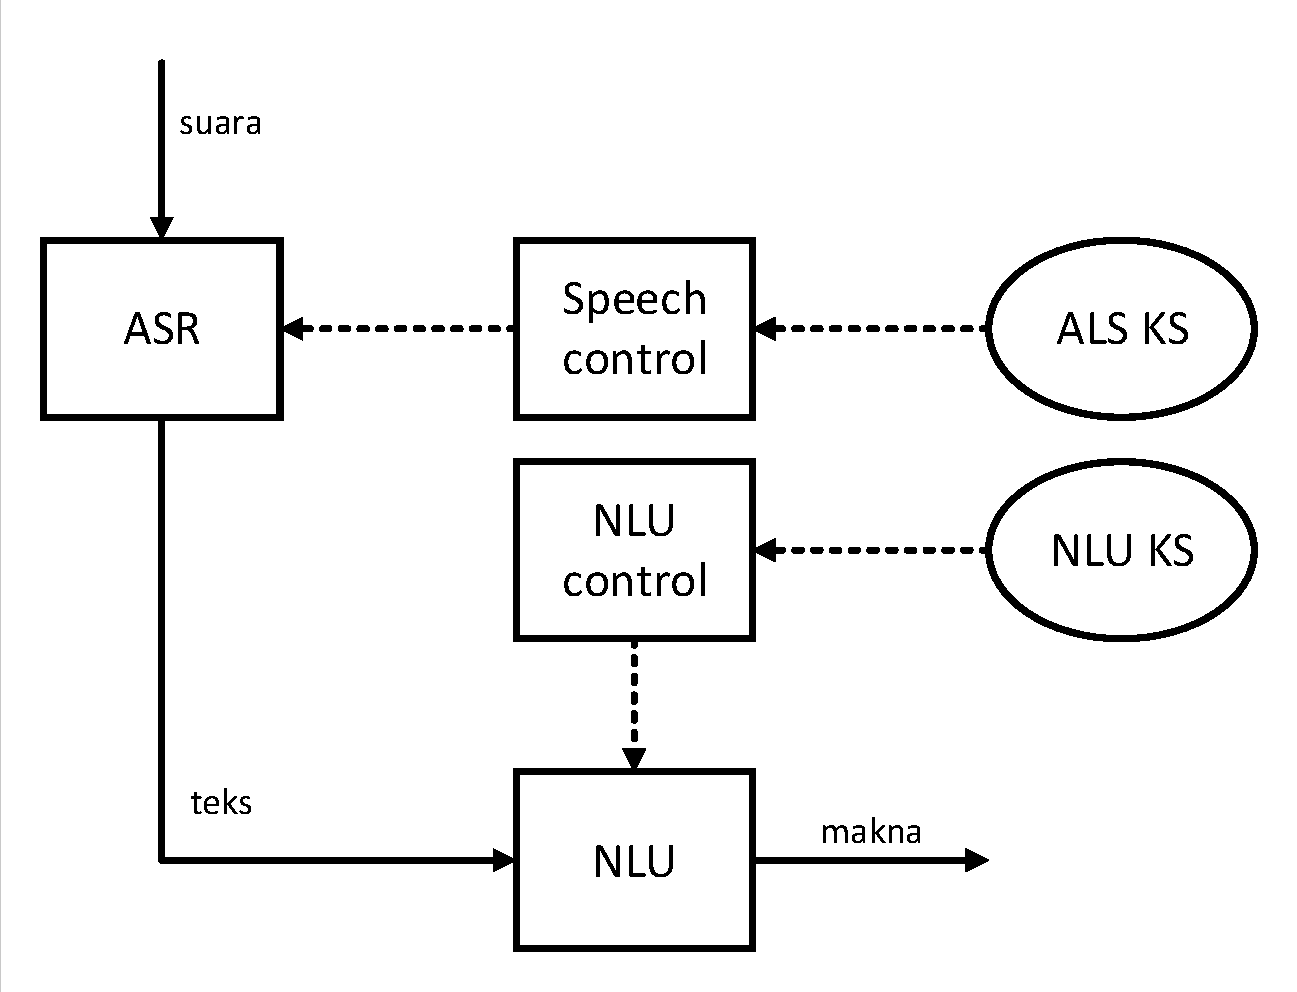
\includegraphics[width=0.5\textwidth, trim=2 2 2 2, clip]{resources/2/early_slu.pdf}
	\caption{Rancangan awal sistem SLU \parencite{tur2011spoken}}
	\label{fig:slu_early}
\end{figure}

Klasifikasi maksud kalimat berarti menentukan sebuah makna dari sebuah kalimat yang diberikan oleh pengguna. Sebagai contoh, kalimat “putarkan sebuah lagu” memiliki makna “putar media” berupa lagu. Makna tersebut kemudian diterjemahkan menjadi sebuah aksi oleh sistem. Makna kalimat bisa didapatkan dengan melihat kata-kata yang terkandung di dalam sebuah kalimat, atau melihat pola urutan kata dalam kalimat tersebut.

Pengisian slot adalah metode untuk mengambil entitas-entitas dari sebuah kalimat biasa. Beberapa aksi terkadang membutuhkan masukan parameter untuk melengkapi aksi tersebut. Masukan parameter didapatkan dari dalam kalimat yang dimasukkan oleh pengguna. Sebagai contoh, “putar lagu separuh aku dari noah” berarti pengguna menginginkan sebuah lagu diputarkan oleh sistem. Namun, permintaan pengguna menjadi lebih spesifik karena pengguna menyebutkan judul lagu beserta artis. Judul lagu adalah “separuh aku” dengan artis adalah “noah”. Metode yang dapat digunakan untuk mengambil entitas adalah melakukan pelabelan kata-kata yang menjadi entitas dengan menggunakan \textit{recurrent neural network} (RNN).

\subsection{\textit{Machine Learning}}

Pembelajaran mesin, atau \textit{machine learning}, adalah sebuah program komputer yang dirancang untuk belajar dari pengalaman dengan acuan berupa kelas tugas-tugas dan pengukuran performa, jika performa pada suatu tugas, yang telah diukur, diperbaiki dengan pengalaman \parencite{mitchell1997machine}. Pembelajaran mesin menggunakan data-data yang telah terkumpul untuk membentuk sebuah pola yang dapat digunakan pada data yang akan muncul atau dimasukkan oleh pengguna.

Pembelajaran mesin diterapkan pada berbagai macam aplikasi, yang ditujukan untuk mengurangi peran manusia dalam melakukan hal tersebut. Sebagai contoh, pembelajaran mesin digunakan untuk melakukan klasifikasi gambar, teks, suara, dan lain-lain. Selain itu, pembelajaran mesin diaplikasikan ke dalam analisis data dengan jumlah yang sangat besar atau biasa disebut sebagai \textit{big data}.

\subsection{\textit{Artificial Neural Network} (ANN)}

\textit{Artificial neural network} (ANN) adalah sistem komputasi yang memiliki elemen-elemen pemrosesan sederhana yang saling terhubung, yang mana dapat memproses informasi dengan respon keadaan dinamisnya kepada masukan dari luar \parencite{caudill1987neural}. Gambar \ref{} menggambarkan rupa dari ANN paling dasar. ANN terdiri dari tiga jenis lapisan, yaitu lapisan masukan, lapisan tersembunyi, serta lapisan keluaran. Lapisan masukan adalah lapisan yang berisi nilai-nilai masukan berasal dari data yang telah terkumpul. Lapisan tersembunyi berisi fungsi-fungsi aktivasi yang digunakan untuk menentukan keluaran yang diinginkan oleh \textit{neural network} secara keseluruhan.

\textit{Neural network} memiliki banyak variasi untuk kondisi data yang berbeda-beda. Jenis \textit{neural network} yang sangat dasar adalah \textit{feed forward neural network}, digunakan untuk melakukan klasifikasi sederhana. Untuk laporan ini, jenis \textit{neural network} yang digunakan adalah \textit{neural network} yang dapat digunakan dalam melakukan klasifikasi sekuensial, seperti \textit{recurrent neural network} (RNN) dan \textit{convolutional neural network} (CNN).

\subsection{\textit{Convolutional Neural Network} (CNN)}

\textit{Convolutional neural network} atau CNN biasa digunakan untuk mengenali objek-objek yang berada di dalam sebuah gambar. CNN mencoba memprediksi sebuah objek yang bersangkutan dengan mendeteksi fitur-fitur yang terdapat dalam sebuah gambar menggunakan \textit{filter}. Untuk penerapan di dalam teks, fitur-fitur tersebut didapatkan dengan melakukan \textit{embedding} pada sebuah kata yang bersangkutan. \textit{Embedding} adalah proses untuk merepresentasikan sebuah kata menjadi vektor multi dimensi.

Keuntungan yang dimiliki oleh CNN, jika dibandingkan dengan \textit{recurrent neural network} (RNN), adalah kemampuan CNN dalam melihat kata yang berada di depan satu kata yang sedang dilatih. Dengan begitu, CNN dapat mempertimbangkan kata sebelum dan kata selanjutnya untuk memasangkan label pada sebuah kata.

\subsection{\textit{Long Short Term Memory} (LSTM)}

\textit{Long short term memory} atau LSTM digunakan untuk mengatasi permasalahan latihan dengan menggunakan data yang bersifat \textit{sequential}. LSTM digunakan untuk mengatasi kelemahan yang dimiliki oleh RNN, yaitu RNN tidak mampu menyimpan informasi dalam jangka waktu yang sangat lama. LSTM dapat memutuskan apakah sebuah informasi akan diteruskan pada iterasi berikutnya atau dilupakan dengan bantuan dari gerbang pelupa (\textit{forget gate}).

Gambar \ref{fig:lstm} menunjukkan isi dari sebuah sel LSTM. Sel LSTM terdiri dari empat jenis gerbang, yaitu dua gerbang masukan, gerbang keluaran, dan gerbang pelupa. Semua gerbang mengandalkan masukan yang berasal dari masukan kata iterasi saat ini dan luaran dari iterasi sebelumnya. Kedua gerbang masuk mengolah nilai luaran dan masukan dengan menggunakan fungsi aktivasi sigmoid dan tanh, kemudian dilakukan operasi perkalian matriks pada kedua hasil tersebut. Gerbang pelupa mengolah kedua nilai dengan menggunakan fungsi aktivasi sigmoid. Terakhir, gerbang luaran mengolah kedua nilai dengan menggunakan fungsi aktivasi sigmoid. Kemudian terdapat sebuah nilai yang disebut dengan nilai keadaan sel. Nilai keadaan sel saat ini didapatkan dengan mengalikan nilai keadaan sel sebelumnya dengan nilai luaran gerbang pelupa, lalu ditambahkan dengan hasil dari kedua gerbang masukan.

\begin{figure}[H]
	\centering
	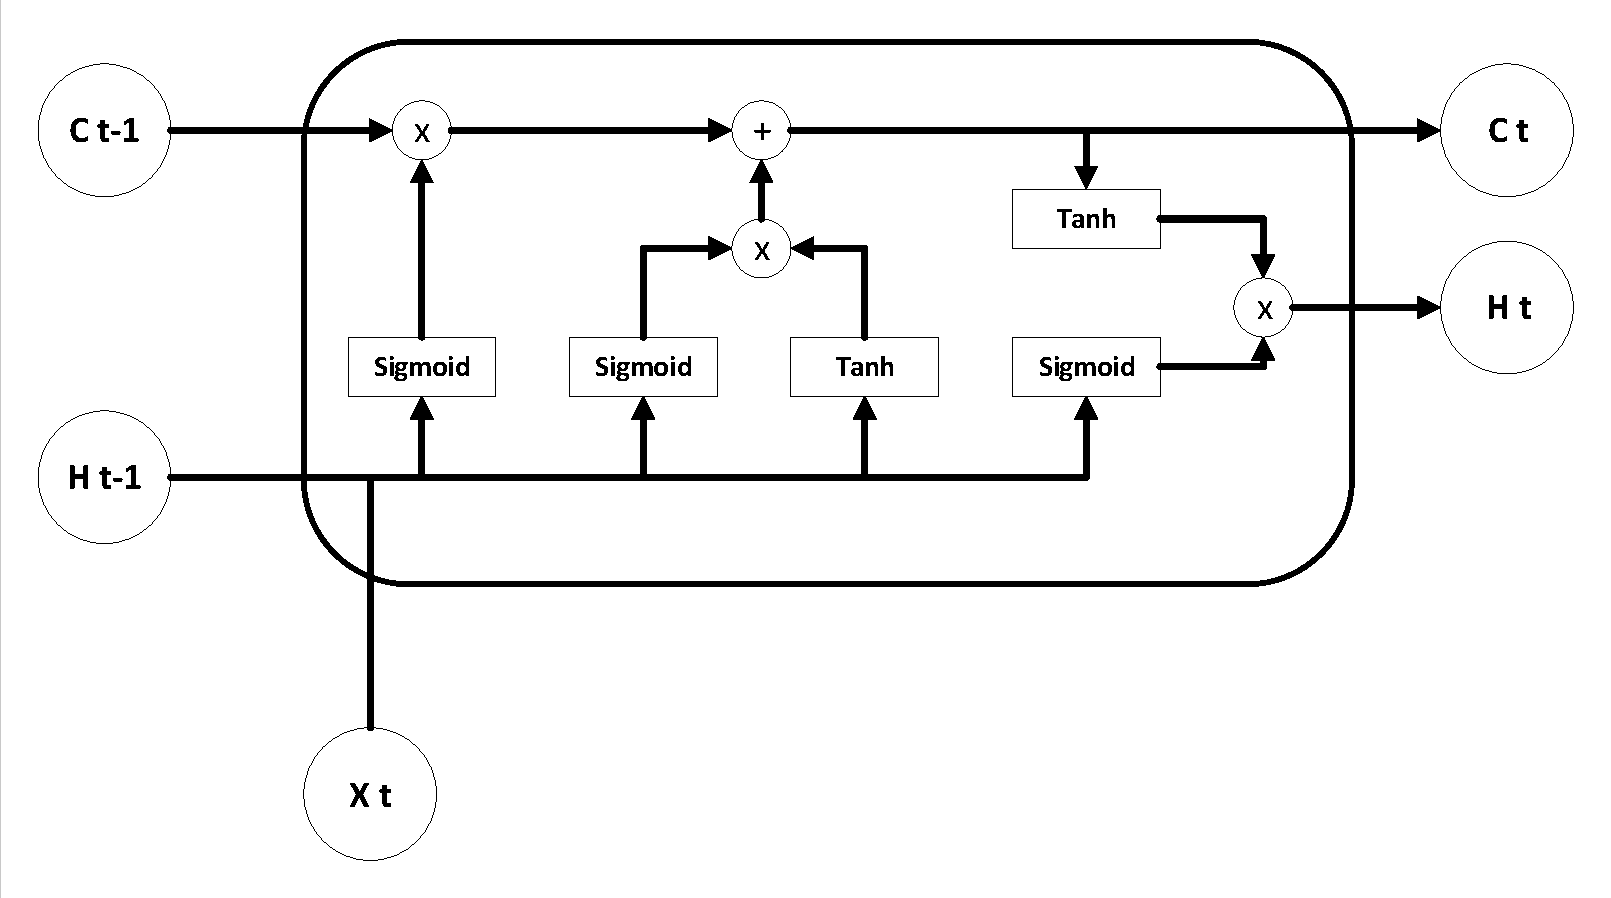
\includegraphics[width=0.8\textwidth, trim=2 2 2 2, clip]{resources/2/lstm.pdf}
	\caption{Arsitektur sel LSTM}
	\label{fig:lstm}
\end{figure}

\section{Analisis Produk}

Produk terkait yang menjadi acuan dalam pengerjaan Tugas Akhir adalah Rasa NLU, produk NLU \textit{open source} yang dibangun oleh Rasa HQ.

\subsection{Alat-Alat yang Digunakan}

Rasa NLU merupakan salah satu bagian dari Rasa Stack, \textit{library} Python yang digunakan untuk membangun sistem \textit{chatbot} berbasis NLU. Rasa NLU membutuhkan komponen-komponen sebagai berikut: spaCy sebagai \textit{library} pembantu Rasa NLU dalam melakukan pengolahan teks, dan fastText sebagai model vektor kata yang digunakan untuk membantu spaCy dalam mengolah teks.

\subsubsection{Rasa}

Rasa, terdiri dari Rasa NLU dan Rasa Core, adalah sepasang \textit{open-source library} Python yang digunakan untuk membangun perangkat lunak berbasis percakapan \parencite{bocklisch2017rasa}. Rasa biasanya digunakan untuk pengembangan robot percakapan atau dikenal dengan \textit{chatbot} berbentuk teks. Tujuan dari Rasa adalah membantu para pengembang untuk mengembangkan manajemen dialog dan pemahaman bahasa berdasarkan pembelajaran mesin. Pengembangan Rasa terinspirasi dari beberapa \textit{library} yang telah ada, seperti scikit-learn dan Keras untuk API, fastText untuk klasifikasi teks, dan GloVe untuk penyediaan data latih untuk \textit{word embedding}. Versi Rasa yang digunakan dalam pengerjaan Tugas Akhir, yaitu Rasa NLU versi 0.11.4 dan Rasa Core versi 0.8.6.

Arsitektur Rasa dapat dilihat pada Gambar \ref{fig:rasa_arch}. Terdapat empat bagian di dalam arsitektur Rasa, yaitu \textit{Interpreter, Tracker, Policy}, dan \textit{Action}. Bagian Interpreter ditangani oleh Rasa NLU, sedangkan bagian yang lain ditangani oleh Rasa Core. Rasa bersifat modular, sehingga \textit{library} dapat diintegrasikan dengan \textit{library} lain, seperti Rasa Core dapat dihubungkan dengan \textit{Interpreter} selain Rasa NLU, dan sebaliknya.

Tahap-tahap proses yang ada di dalam arsitektur Rasa dapat dijelaskan sebagai berikut. Pertama, pesan yang dimasukkan oleh pengguna dikirimkan ke \textit{Interpreter}. Di dalam \textit{Interpreter} dilakukan proses untuk mengekstrasi \textit{intent}, entities, dan beberapa informasi terstruktur lain dari pesan yang telah dimasukkan. Kedua, luaran dari \textit{Interpreter} diteruskan menuju \textit{Tracker}. \textit{Tracker} akan melacak \textit{state} dari percakapan dan memberikan pemberitahuan baru bahwa pesan telah diterima oleh \textit{Tracker}. Ketiga, \textit{Policy} menerima  \textit{state} dari \textit{Tracker}. Keempat, \textit{Policy} menentukan \textit{Action} yang harus dilakukan sebagai tanggapan pesan dari pengguna.Kelima, \textit{Action} yang terpilih dicatat oleh \textit{Tracker}. Terakhir, \textit{Action} mulai dieksekusi kepada pengguna, baik berupa pencarian atau mengeluarkan pesan.

\begin{figure}[H]
	\centering
	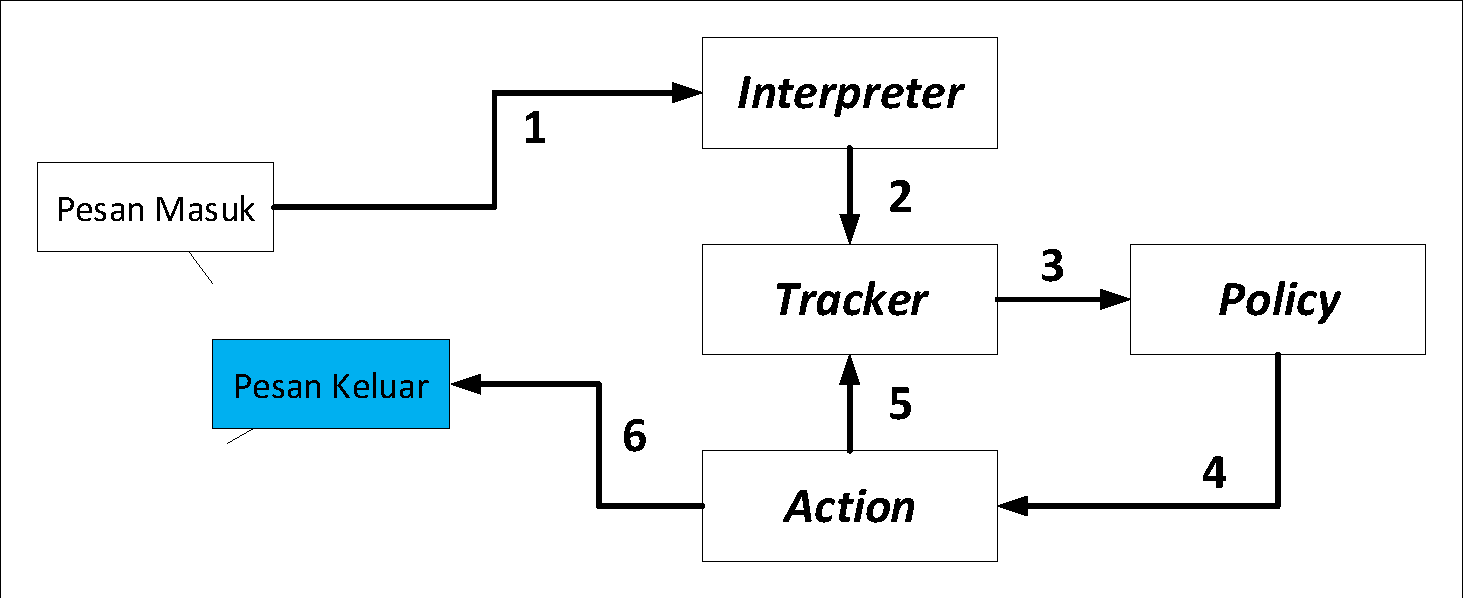
\includegraphics[width=0.9\textwidth, trim=2 2 2 2, clip]{resources/2/rasa_arch.pdf}
	\caption{Bagan arsitektur Rasa \parencite{bocklisch2017rasa}}
	\label{fig:rasa_arch}
\end{figure}

Secara sederhana, cara Rasa bekerja ditunjukkan oleh bagan pada Gambar \ref{fig:rasa_process}. Terdapat tiga proses utama dari Rasa NLU dan Rasa Core, yaitu melatih NLU, melatih dialog, dan menjalankan agen dialog.

\begin{figure}[H]
	\centering
	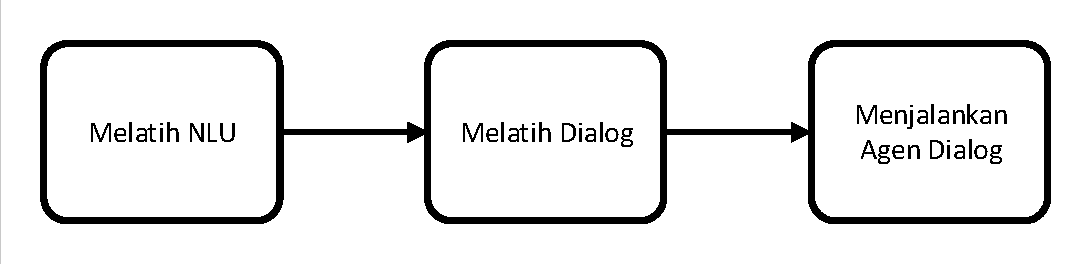
\includegraphics[width=0.8\textwidth, trim=2 2 2 2, clip]{resources/2/rasa_process.pdf}
	\caption{Bagan proses utama Rasa}
	\label{fig:rasa_process}
\end{figure}

\begin{enumerate}[label=\textit{\Alph*)}, itemindent=*, series=rasa_process_list]
	\item \textit{Melatih NLU}
\end{enumerate}

Pelatihan NLU dilakukan oleh Rasa NLU dengan bantuan pengolah teks seperti spaCy dan MITIE. Pelatihan NLU berguna untuk melatih sistem untuk dapat memahami teks dan entitas didalamnya yang akan dimasukkan oleh pengguna dan menyimpan model latihan untuk digunakan saat agen dialog siap untuk dijalankan.

Untuk dapat menjalankan proses ini, dibutuhkan dua data masing-masing dalam berbentuk file JSON, yaitu data latihan dan data konfigurasi. Data latihan berisi teks masukan yang dijadikan contoh, maksud dari teks tersebut, serta entitas yang terkandung di dalamnya. Sedangkan data konfigurasi berisikan konfigurasi yang digunakan sebagai acuan dalam melatih NLU, seperti bahasa, pipeline yang digunakan untuk latihan, lokasi data latihan, dan lain-lain.

Proses-proses untuk melatih NLU dapat dilihat pada Gambar \ref{fig:rasaNLU_train}, dan penjelasan tiap proses adalah sebagai berikut:

\begin{enumerate}
	\item Rasa NLU mengambil data konfigurasi, setelah itu mengambil data latihan,
	\item memuat data latihan dan mengubahnya menjadi obyek TrainingData,
	\item memuat data konfigurasi dan mengubahnya menjadi obyek RasaNLUConfig,
	\item membuat obyek Trainer sebagai “pelatih” dan mempersiapkan obyek tersebut dengan menggunakan obyek RasaNLUConfig sebagai masukan,
	\item memanggil prosedur latihan pada obyek Trainer dengan menggunakan obyek TrainingData sebagai masukan, dan,
	\item menyimpan model hasil latihan menuju direktori sistem.
\end{enumerate}

\begin{figure}[H]
	\centering
	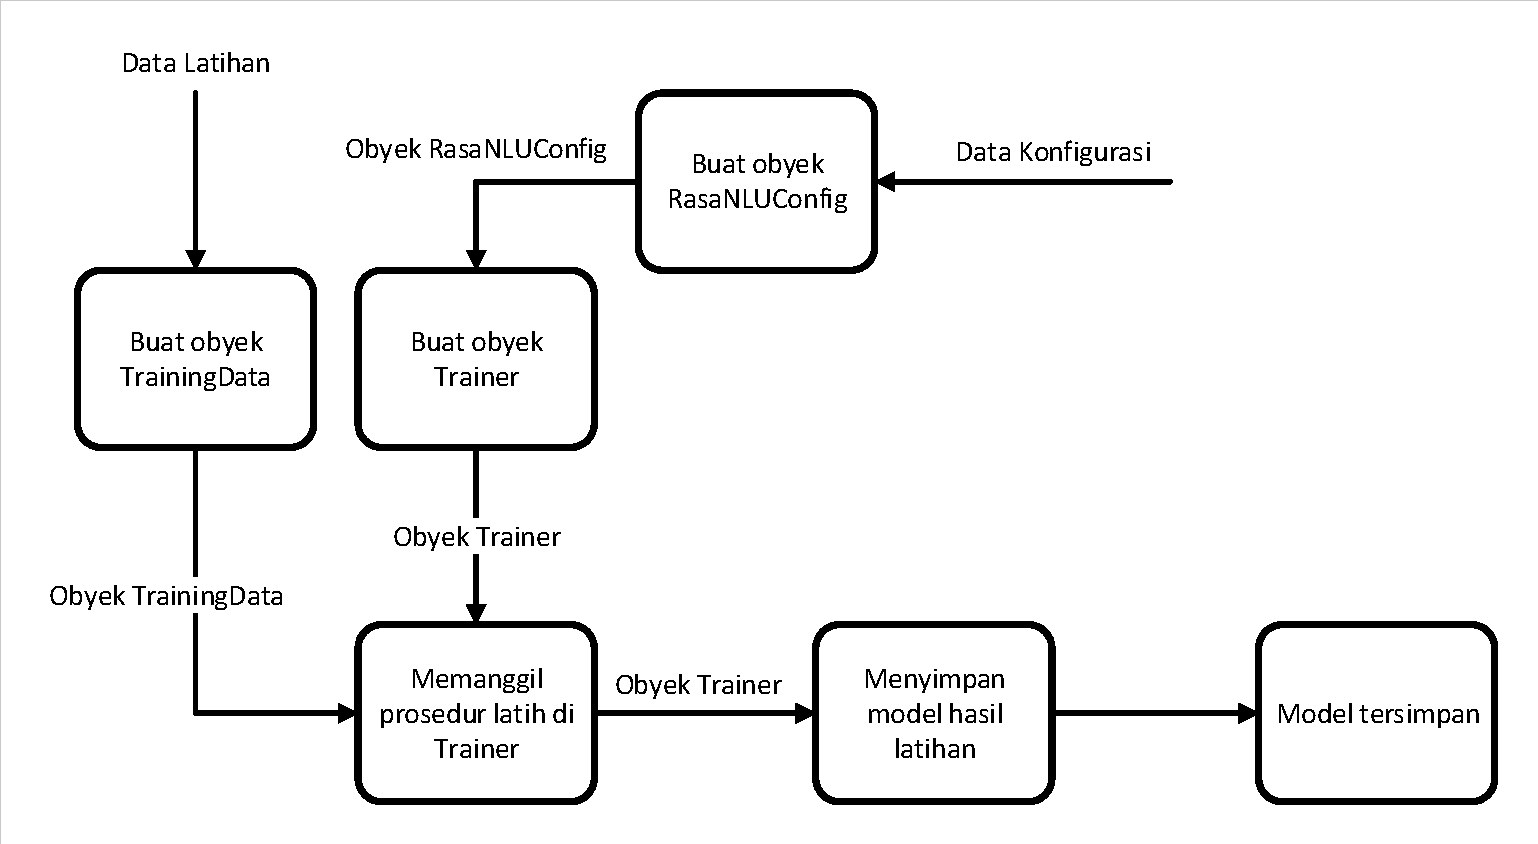
\includegraphics[width=0.8\textwidth, trim=2 2 2 2, clip]{resources/2/rasaNLU_train.pdf}
	\caption{Bagan alur latihan NLU dari Rasa NLU}
	\label{fig:rasaNLU_train}
\end{figure}

Di dalam data konfigurasi, terdapat pengaturan \textit{pipeline} yang digunakan untuk mengatur data latihan akan dilatih dengan menggunakan komponen apa saja. Alur persiapan \textit{pipeline} yang digunakan adalah, pertama menginisiasi semua komponen, lalu melakukan latihan jika terdapat prosedur latihan didalamnya, dan terakhir menyimpan hasil latihan per komponen ke dalam direktori sistem. Dalam pengerjaan Tugas Akhir ini, \textit{pipeline template} yang digunakan adalah spacy\_sklearn yang berisikan komponen latih sebagai berikut:

\begin{enumerate}
	\item nlp\_spacy, digunakan untuk inisialisasi spaCy sebelum menggunakan komponen latih spaCy yang lain,
	\item tokenizer\_spacy, digunakan untuk melakukan tokenisasi dari teks masukan dengan menggunakan tokenisasi dari spaCy,
	\item intent\_featurizer\_spacy, digunakan untuk membuat definisi ekstrasi fitur dari teks masukan dengan menggunakan spaCy. Fitur tersebut akan digunakan untuk melakukan klasifikasi maksud kalimat,
	\item intent\_entity\_featurizer\_regex, digunakan untuk mencatatkan seluruh \textit{regular expressio}n yang telah didefinisikan dalam data latihan,
	\item ner\_crf, digunakan untuk melakukan pengenalan entitas dengan menggunakan metode latihan \textit{conditional random field} (CRF) yang disediakan oleh \textit{library} sklearn-crfsuite,
	\item ner\_synonym, digunakan untuk menampung teks-teks yang memiliki nilai entitas yang sama, dan,
	\item intent\_classifier\_sklearn, digunakan untuk melakukan latihan klasifikasi maksud kalimat dengan masukan berupa fitur teks yang telah dilakukan oleh intent\_featurizer\_spacy. Latihan klasifikasi dilakukan dengan menggunakan \textit{support vector machine} (SVM) dan pengaturan parameter latih menggunakan metode \textit{grid-search} yang disediakan oleh scikit-learn.
\end{enumerate}

\begin{enumerate}[resume*=rasa_process_list]
	\item \textit{Melatih Dialog}
\end{enumerate}

Pelatihan dialog dilakukan dengan menggunakan Rasa Core. Pelatihan dialog berguna untuk mendefinisikan domain NLU dari sistem serta melatih agen dialog untuk menciptakan prediksi respon yang tepat berdasarkan masukan dari pengguna sebelumnya. Prediksi didapatkan dengan menggunakan sebuah komponen yaitu \textit{policy}.

Untuk dapat menjalankan proses ini, dibutuhkan dua data masing-masing dalam bentuk file \textit{markdown} dan YML, yaitu data cerita dan data domain. Data cerita digunakan untuk mengkonstruksi alur percakapan yang mungkin terjadi antara pengguna dengan sistem. Data cerita terdiri dari balok-balok cerita, berisi maksud kalimat yang diekstraksi dari teks masukan pengguna dan respon sistem terhadap masukan tersebut. Jumlah respon dan timbal balik dalam satu balok cerita tidak terbatas. Data domain digunakan untuk inisialisasi definisi dari maksud kalimat, entitas yang terlibat, slot yang tersedia, serta aksi yang akan dilakukan oleh sistem.

Proses-proses untuk melatih agen dialog dijelaskan sebagai berikut:

\begin{enumerate}
	\item Rasa Core mengambil data domain dan data cerita,
	\item membuat agen dialog dengan membuat obyek Agent menggunakan masukan data domain dan policy yang digunakan,
	\item memanggil prosedur latih dari obyek Agent dengan menyertakan data cerita sebagai masukan. Prosedur ini juga membuat obyek PolicyTrainer dan melakukan pelatihan, dan,
	\item menyimpan agen dialog terlatih ke dalam direktori sistem.
\end{enumerate}

\begin{enumerate}[resume*=rasa_process_list]
	\item \textit{Menjalankan Agen Dialog}
\end{enumerate}

Setelah model NLU dan agen dialog telah tersimpan ke dalam direktori, sistem sudah siap untuk menjalankan agen dialognya. Sistem akan melakukan \textit{loop} selamanya terhadap proses memasukkan teks. Teks yang telah dimasukkan oleh pengguna akan diprediksi maksud kalimatnya sehingga sistem dapat menentukan aksi yang tepat.

\subsubsection{spaCy}

spaCy adalah sebuah \textit{open-source library} Python digunakan untuk melakukan pengolahan teks, khususnya NLP, dalam tingkat industri \parencite{spacy2}. spaCy mendukung banyak bahasa selain MITIE, dan lebih mudah untuk menambahkan bahasa baru, cukup dengan menyediakan model bahasa yang dibutuhkan ke dalam spaCy. Versi spaCy yang digunakan adalah versi 2.0.11.

Arsitektur spaCy dapat terlihat di dalam Gambar \ref{fig:spaCy_arch} \parencite{spacy2}. Terdapat dua struktur data pusat yang berada di dalam spaCy, yaitu Doc dan Vocab. Doc berisi rangkaian dari \textit{token} dan semua anotasinya, sedangkan Vocab berisi sekumpulan tabel \textit{look-up} untuk menyediakan informasi umum ke seluruh dokumen, bertujuan untuk mencegah terjadinya duplikasi data dan memastikan bahwa fakta hanya tersimpan di dalam satu sumber.

Dengan menyimpan semua fakta di dalam satu sumber dapat menghemat penyimpanan di dalam arsitektur spaCy itu sendiri. Seperti, Doc menyimpan seluruh data-data anotasi teks, sedangkan Token dan Span hanya berupa \textit{view} yang berisi \textit{pointer} untuk merujuk kepada data yang ada di Doc.

\begin{figure}[H]
	\centering
	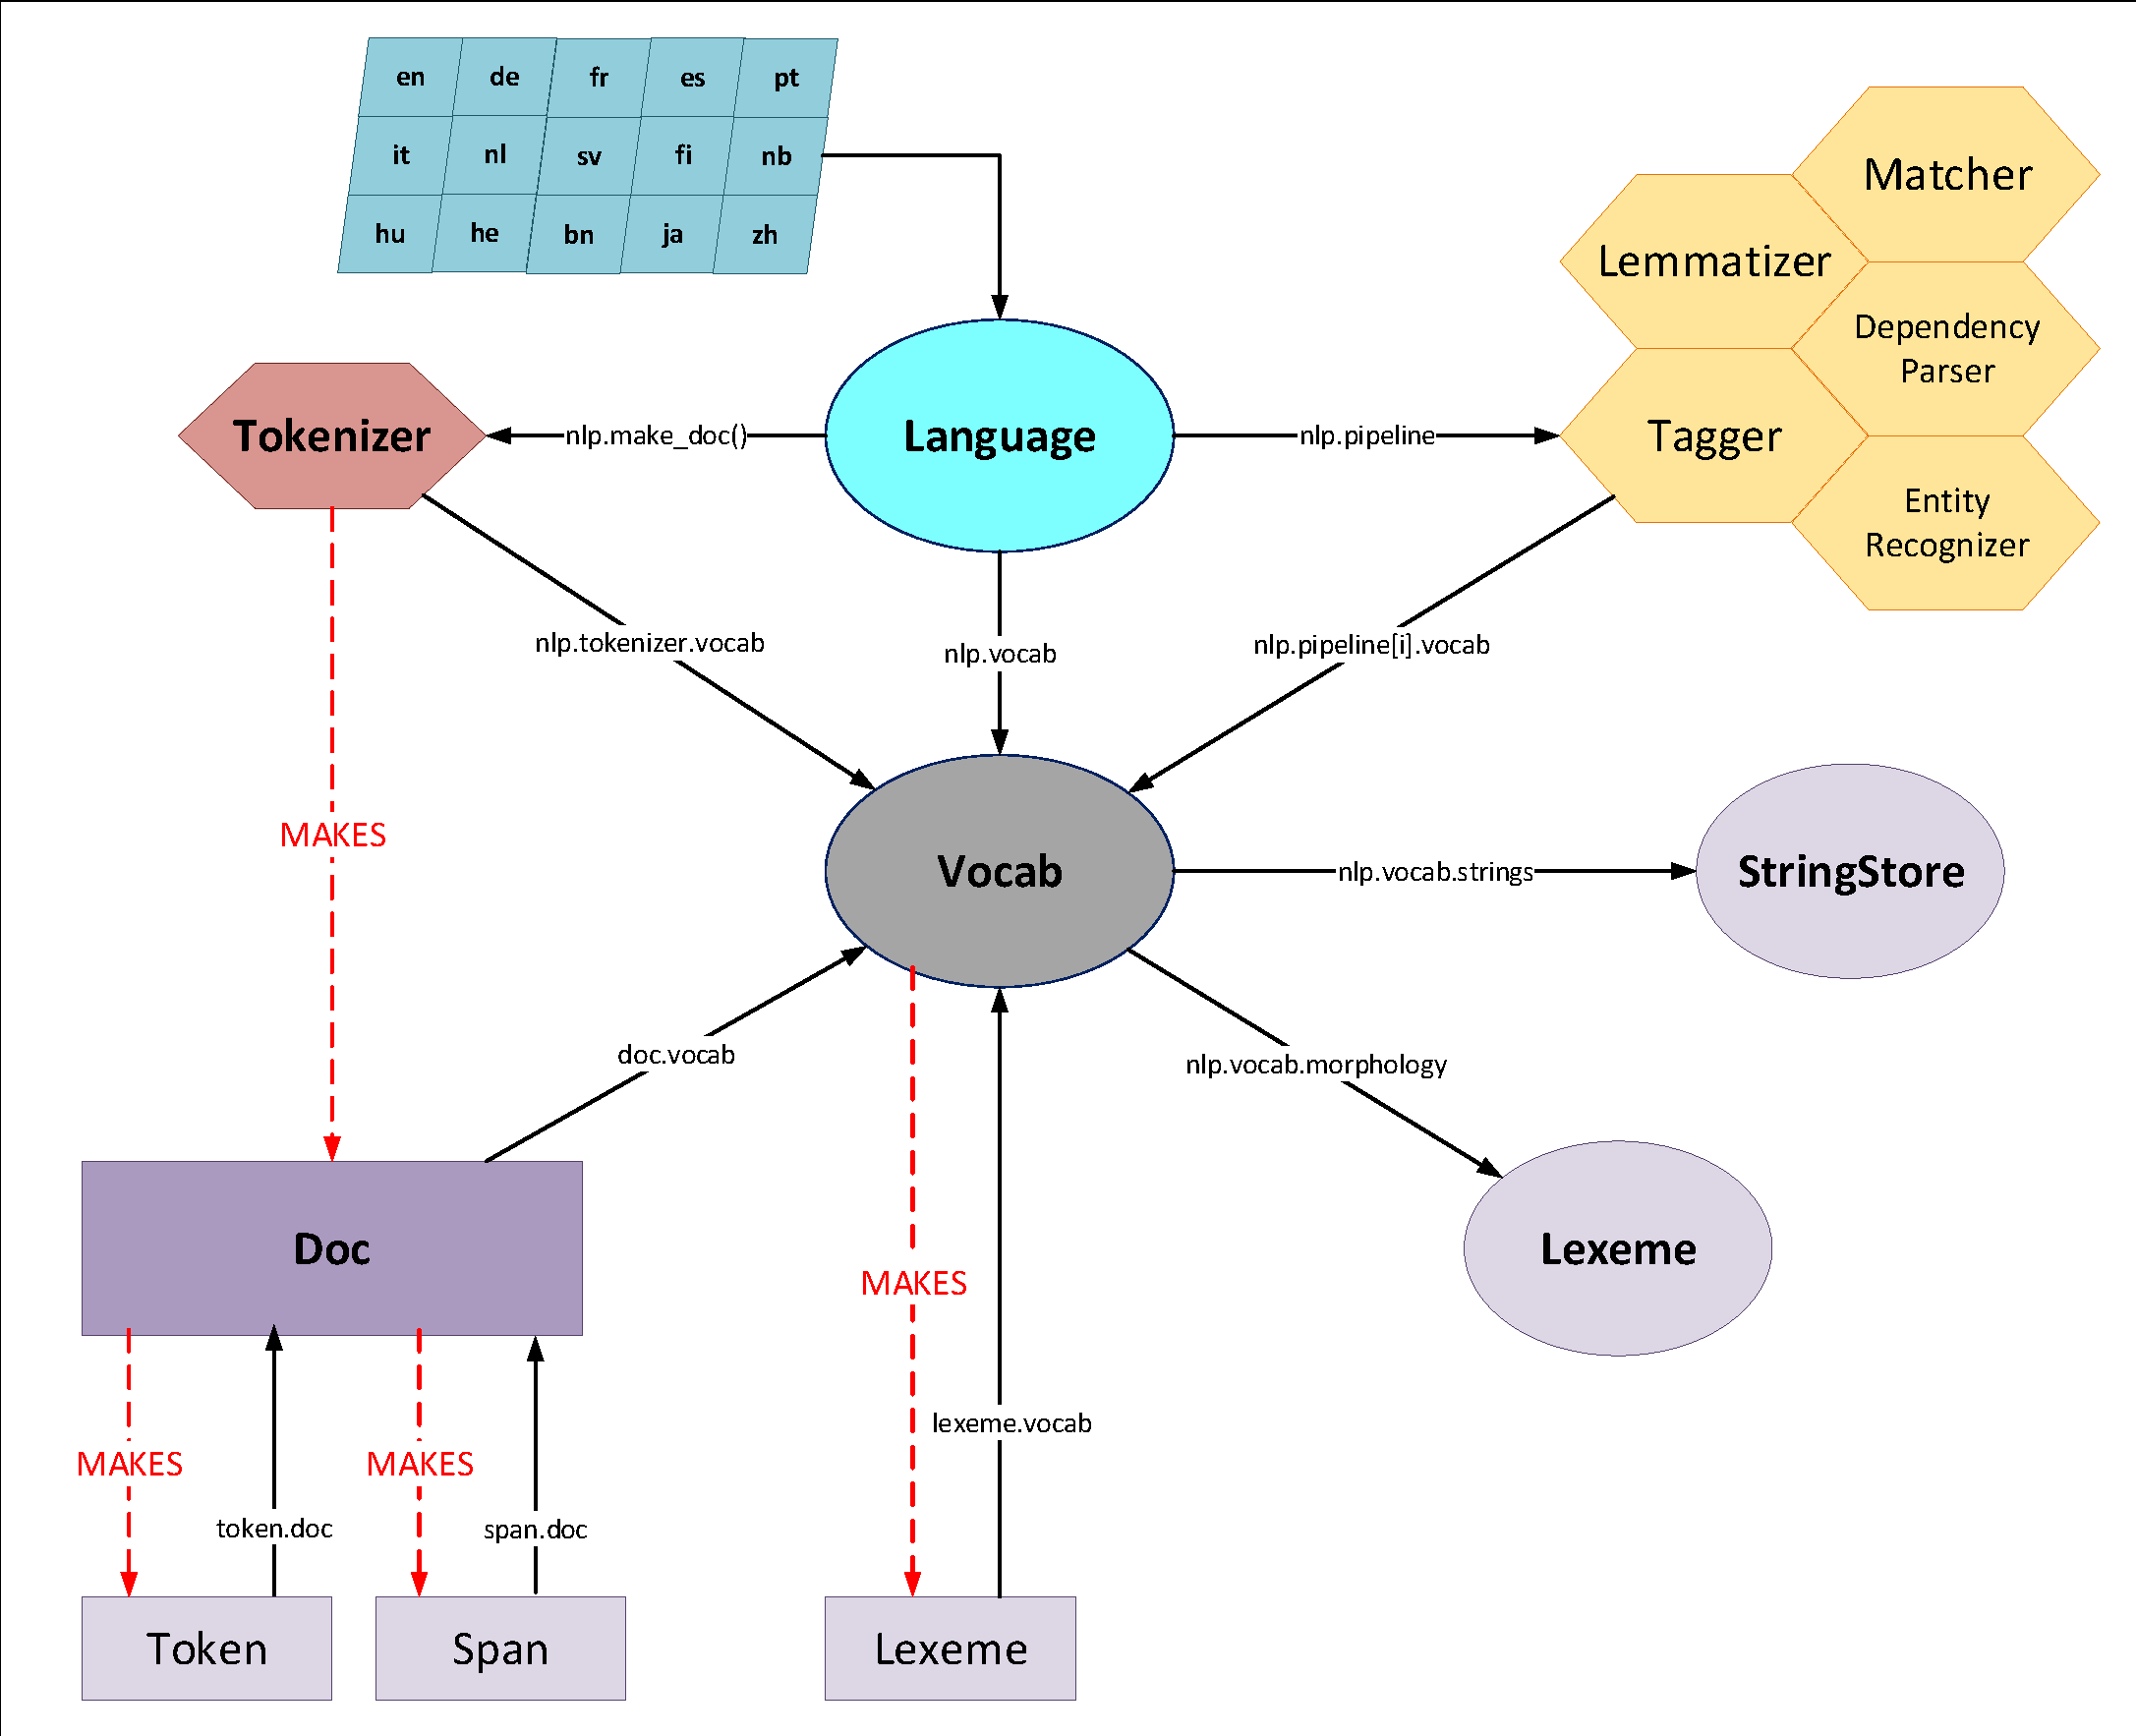
\includegraphics[width=0.9\textwidth, trim=2 2 2 2, clip]{resources/2/spacy_arch.pdf}
	\caption{Bagan arsitektur spaCy \parencite{spacy2}}
	\label{fig:spaCy_arch}
\end{figure}

\subsubsection{fastText}

fastText adalah \textit{library} untuk klasifikasi dan representasi teks yang dibangun oleh peneliti AI dari Facebook \parencite{joulin2017bag}. Pemrosesan yang dilakukan adalah mengubah sebuah kalimat-kalimat yang tersedia menjadi sebuah model vektor. Model vektor merepresentasikan kedekatan antara suatu kata dengan kata yang lain, memiliki nilai rentang antara 0 hingga 1. Model vektor tersebut dapat dipakai tidak hanya oleh \textit{library} fastText, namun juga dapat digunakan oleh \textit{library} luar, seperti spaCy.

Untuk pengerjaan Tugas Akhir ini, digunakan model vektor yang telah tersedia oleh fastText di dalam repositori GitHub. Model vektor yang digunakan adalah model vektor berbahasa Indonesia, yang diproses dari teks-teks yang tersedia di Wikipedia. Untuk dapat menggunakan model vektor, terlebih dahulu model vektor dikonversi menjadi model bahasa spaCy, dalam hal ini model bahasa Indonesia.

\subsection{Teori yang Diterapkan}

\subsubsection{Pengenalan Entitas dengan \textit{Conditional Random Field}}

\textit{Conditional random field} (CRF) adalah metode pembelajaran yang digunakan untuk data-data yang bersifat berurutan. CRF menggunakan fitur-fitur yang dimiliki oleh sebuah kata untuk melakukan pelatihan. Fitur yang digunakan untuk CRF dapat bervariasi sesuai kebutuhan, namun fitur dasar yang tersedia adalah kata utama dan kata sebelum kata utama. CRF biasanya digunakan untuk \textit{sequence labelling} teks.

Rasa NLU menggunakan \textit{library} Python yaitu sklearn-crfsuite. \textit{Library} ini merupakan pembungkus \textit{library} python-crfsuite yang mana menyediakan \textit{estimator} yang cocok dengan scikit-learn \parencite{sklearncrf}. Hal tersebut memudahkan penggunaan model CRF untuk pelatihan dan menyimpan model hasil latihan. Selain itu, spaCy juga menyediakan fitur yang dapat digunakan oleh CRF milik Rasa NLU, yaitu fitur POS \textit{tag} untuk tiap kata dalam kalimat.

\subsubsection{Klasifikasi Maksud Kalimat dengan \textit{Support Vector Machine}}

\textit{Support vector machine} (SVM), atau \textit{support vector network}, adalah sebuah metode pembelajaran yang memetakan vektor masukan menjadi ruang fitur dengan dimensi yang tinggi melalui pemetaan non linear yang telah dipilih sebelumnya \parencite{cortes1995support}. SVM biasanya digunakan untuk menjelaskan kegiatan klasifikasi dengan metode support vector, namun kegunaan SVM juga bisa digunakan untuk kegiatan regresi. Oleh karena itu, SVM terbagi menjadi dua, yaitu \textit{support vector classification} (SVC) untuk klasifikasi dan \textit{support vector regression} (SVR) untuk regresi \parencite{gunn1998support}.

Rasa NLU menggunakan SVM untuk melakukan klasifikasi maksud kalimat dari scikit-learn. Dengan jumlah maksud kalimat yang berjumlah lebih dari dua, maka scikit-learn akan menggunakan metode-metode untuk mengakali SVM sehingga dapat digunakan untuk kasus melakukan klasifikasi lebih dari dua kelas. Selain itu, Rasa menggunakan metode \textit{grid-search} untuk melakukan \textit{hyperparameter tuning.}

\subsection{Analisis Kekurangan Sistem}

Selama pengerjaan sistem NLU berlangsung, terdapat kekurangan-kekurangan yang dimiliki oleh alat-alat yang digunakan untuk membangun sistem. Kekurangan tersebut berkaitan dengan permasalahan proyek yang sedang dikerjakan.

%\subsubsection{Model yang Digunakan Tidak Cukup}
%
%Model vektor fastText digunakan untuk dapat membangun model bahasa Indonesia spaCy, dan digunakan dalam melakukan pengolahan teks di Rasa. Namun, model bahasa yang berhasil dibangun dari model vektor hanyalah pada bagian kosakata saja. Untuk dapat membangun model bahasa yang baik, model juga memerlukan bagian-bagian seperti \textit{named entity recognition}, \textit{parser}, serta \textit{tagger}.
%
%\textit{Named entity recognition}, atau NER, merujuk kepada pengenalan \textit{token-token} yang merupakan sebuah entitas, seperti nama oganisasi, nama tempat, tanggal, waktu, angka urutan, dan lain-lain. NER diperlukan untuk membedakan antara \textit{token} biasa dengan \textit{token} entitas. \textit{Parser} merujuk kepada \textit{dependency parsing} yaitu melihat ketergantungan sebuah token dengan token yang lain. Sebagai contoh, kalimat “Budi memakan nasi” memiliki dua ketergantungan, yaitu “Budi” memiliki ketergantungan subyek dengan “memakan”, dan “nasi” memiliki ketergantungan obyek dengan “memakan”. Terakhir, \textit{tagger} merujuk kepada \textit{POS tagging} yaitu memberikan tanda kepada token berdasarkan sifat kata dari token tersebut, misal kata kerja, kata benda, tanda baca, dan lain-lain.
%
%Terdapat beberapa korpus untuk latihan yang menyediakan komponen seperti \textit{dependency parser} dan \textit{POS tag}, salah satunya berasal dari Universal Dependencies. Universal Dependencies menyediakan korpus yang diambil dari berbagai sumber, seperti berita, artikel blog, istilah hukum, istilah medis, Wikipedia, dan lain-lain.
%
\subsubsection{Kebutuhan Ekstraksi Fitur untuk CRF}

CRF membutuhkan fitur-fitur yang telah didefinisikan sebelumnya untuk dapat melakukan latihan, seperti CRF yang diterapkan oleh Rasa membutuhkan fitur POS \textit{tag} pada sebuah kata. Fitur tersebut hanya bisa didapatkan dengan \textit{library} NLP, seperti spaCy, yang dapat melakukan latihan POS \textit{tag} berdasarkan model yang telah disediakan oleh pengguna. Oleh karena itu, sebuah kalimat masukan perlu melakukan klasifikasi dengan spaCy terlebih dahulu sebelum akhirnya diekstraksi dengan menggunakan Rasa.

Model vektor fastText digunakan untuk dapat membangun model bahasa Indonesia spaCy, dan digunakan dalam melakukan pengolahan teks di Rasa. Namun, model bahasa yang berhasil dibangun dari model vektor hanyalah pada bagian kosakata saja. Untuk dapat membangun model bahasa yang baik, model juga memerlukan bagian-bagian seperti POS \textit{tagger}. Kekurangan informasi tersebut berakibat pada klasifikasi spaCy yang menjadi tidak maksimal.

Lalu, model dari fastText hanya tersedia dalam bahasa Indonesia yang baku. Hal ini dapat menyebabkan kesulitan dalam mengenal kata-kata yang baru diucapkan, atau kata yang tidak baku seperti kata-kata dalam percakapan sehari-hari. Oleh karena itu, pendekatan CRF dari Rasa NLU tidak cocok untuk digunakan pada proyek ini.

%\subsubsection{Penggunaan SVM untuk Klasifikasi Lebih dari Dua Kelas}
%
%Rasa NLU menggunakan metode SVM dengan tambahan pengaturan grid-search dari scikit-learn untuk melakukan pelatihan klasifikasi maksud kalimat. Kelemahan yang terdapat pada SVM dalam melakukan klasifikasi adalah SVM hanya dapat melakukan klasifikasi pada dua kelas saja. SVM tidak dirancang untuk mengatasi permasalahan klasifikasi yang membutuhkan lebih dari dua kelas. Namun, scikit-learn dapat mengatasi permasalahan tersebut dengan menggunakan skema klasifikasi one-versus-one. Skema tersebut bekerja dengan cara membuat satu alat klasifikasi untuk tiap pasangan kelas yang ada. Pada saat prediksi, kelas yang menerima voting tertinggi akan terpilih [cit].
%
%Kelemahan yang dimiliki oleh skema one-versus-one adalah jumlah klasifikasi yang dilakukan, yaitu (jumlah kelas * (jumlah kelas – 1) / 2) klasifikasi, membuat skema ini memiliki kompleksitas O(jumlah kelas \^{} 2). Dengan jumlah klasifikasi yang banyak, SVM dirasa tidak efisien untuk melakukan klasifikasi dengan jumlah kelas yang banyak. Oleh karena itu, metode klasifikasi yang tepat digunakan untuk mengatasi masalah jumlah kelas lebih dari dua tersebut adalah \textit{neural network}.
%
%Keluaran dari \textit{neural network} dapat diatur sesuai dengan jumlah kelas yang tersedia pada data latihan. Fleksibilitas yang dimiliki oleh \textit{neural network} membuat metode ini dapat melakukan satu model dan satu kali latihan klasifikasi untuk dapat menghasilkan model yang bagus untuk digunakan.